\documentclass[letterpaper]{report}
\author{Prof. Rob Marano}
\usepackage{expl3}
\usepackage[margin=0.75in]{geometry}
\usepackage{amsfonts}
\usepackage{amsthm}
\usepackage{latexsym}
\usepackage{amsmath}
\usepackage{amssymb}
\usepackage{setspace}
\usepackage[normalem]{ulem}
\usepackage{multicol}
\usepackage{multirow}
\usepackage{bytefield}
\usepackage{color}
\usepackage{xcolor}
\usepackage{listings}
\usepackage{chronology}
\usepackage{pdfpages}
\usepackage{forloop}
\usepackage{xparse}
\usepackage{xstring}
\usepackage{listofitems}
\usepackage{courier}
\usepackage{textcomp}
\usepackage{graphicx}
\usepackage{hyperref}
\usepackage{enumerate}

\usepackage{./code/mips}
%
% mycommands.tex
%

\newcommand{\colorbitbox}[4][lrbt]{%
    \rlap{\bitbox[#1]{#3}{\color{#2}\rule{\dimexpr\width-0.4pt}{\dimexpr\height-0.4pt}}}%
    \bitbox[#1]{#3}{#4}}

\definecolor{lightgray}{gray}{0.85}

%
% \ExplSyntaxOn
% \NewDocumentCommand{\loopBin}{m}
%  {
%   % save the input in a variable
%   \tl_set:Nn \mips_getletters { #1 }
%   % replace spaces with \textvisiblespace
%   \tl_replace_all:Nnn \mips_getletters { ~ } { \textvisiblespace }
%   % map the input surrounding each item by parentheses
%   \tl_map_inline:Nn \mips_getletters { ##1 }
%  }
% \tl_new:N \mips_getletters
% \ExplSyntaxOff
%


%
% \newcommand{\binLoop}[1]
% {
%     \begin{bytefield}[boxformatting={\centering\itshape},bitwidth=1.5em,endianness=big]{32}
%     \bitheader{0-31}
%     % \StrLen{#1}
%     \foreach \x in {1,...\StrLen{#1}}
%     {
%         \bitbox{\x,#1{\x}}
%     }
    
%     \end{bytefield}
% }
%

%
 % \NewDocumentCommand{\extract}{mm}
\ExplSyntaxOn
\cs_new:Npn \extract #1 #2
 {
  \str_item:fn { #1 } { #2+1 } % since it starts counting from 1
 }
\cs_generate_variant:Nn \str_item:nn {f}
\ExplSyntaxOff

\ExplSyntaxOn
% \cs_new:Npn \makebitboxes #1 #2
 \NewDocumentCommand{\makebitboxes}{mm}
 {
    \begin{bytefield}[boxformatting={\centering\itshape},bitwidth=1.5em,endianness=big]{\numbits}
    \bitheader{0-{#1 - 1}} \\
    
    \int_step_variable:nnnNn {0}{1}{#1-1}{\tvar}
   {
        % (\tvar,\extract{#2}{\tvar})
        \int_compare:nNnTF { \int_mod:nn {\tvar} { 2 } } = { 0 }
       {% odd box
            \colorbitbox{lightgray}{1}{\extract{#2}{\tvar}}
       }
       { %even box
            \bitbox{1}{\extract{#2}{\tvar}}
       }
   }
   \end{bytefield}
  }
\ExplSyntaxOff
%

\ExplSyntaxOn
% \cs_new:Npn \makebitboxes #1 #2
 \NewDocumentCommand{\makeemptybyteboxes}{m}
 {
    \begin{bytefield}[boxformatting={\centering\itshape},bitwidth=1.5em,endianness=big]{32}
    
    \int_step_variable:nnnNn {0}{1}{#1-1}{\tvar}
   {
        % (\tvar,\extract{#2}{\tvar})
        \int_compare:nNnTF { \int_mod:nn {\tvar} { 2 } } = { 0 }
       {% odd box
            \colorbitbox{lightgray}{4}{}
       }
       { %even box
            \bitbox{4}{}
       }
   }
   \end{bytefield}
  }
\ExplSyntaxOff
%

\ExplSyntaxOn
 \NewDocumentCommand{\makeemptybitboxes}{m}
 {
    \begin{bytefield}[boxformatting={\centering\itshape},bitwidth=1.5em,endianness=big]{\numbits}
    \bitheader{0-{#1 - 1}} \\
    
    \int_step_variable:nnnNn {0}{1}{#1-1}{\tvar}
   {
        % (\tvar,\extract{#2}{\tvar})
        \int_compare:nNnTF { \int_mod:nn {\tvar} { 2 } } = { 0 }
       {% odd box
            \colorbitbox{lightgray}{1}{}
       }
       { %even box
            \bitbox{1}{}
       }
   }
   \end{bytefield}
  }
\ExplSyntaxOff
%
\input{./code/lauracode}
\input{./code/testpoints}

\hypersetup{
    colorlinks=true,
    linkcolor=blue,
    filecolor=magenta,      
    urlcolor=cyan,
    pdftitle={ECE 251 Spring 2026 Mid-Term Exam},
    pdfpagemode=FullScreen,
}
\urlstyle{same}

\pagestyle{empty}
\begin{document}

% *** COVER *** 
\begin{minipage}{0.3\textwidth}
    
\includegraphics[width=1.0in]{../../images/cooper_union_logo.png}
\end{minipage}
\begin{minipage}{0.65\textwidth}
    \raggedleft {\bf Name: } $\underbrace{\hspace{2.5in}}_{\mbox{\tiny by writing my name I affirm to abide by the Cooper Union honor code.}}$
\end{minipage}

\vspace{0.1in}

\centerline{\huge \bf Mid-Term Exam}
\vspace{0.1in}

ECE 251 \textemdash{ Computer Architecture} \hfill
12 March 2026 \hfill

Spring 2026 \hfill
Prof. Rob Marano \hfill

\vspace{0.1in}
\textsc{Take-Home Exam Instructions \& Scheduling:}
\begin{itemize}
    \item \textbf{Scheduling:} Email \underline{and} direct message me on Teams by \textbf{6pm ET Friday, March 13 (tomorrow)} to lock in your testing slot. The testing window is from March 13 through \textbf{Wednesday, March 25}.
    \item \textbf{Taking the Exam:} At your scheduled time, I will send the PDF. You have exactly \textbf{90 minutes} (approved accommodations apply) to complete 6 problems (100~pts), \textbf{open book WITHOUT use of the internet or a generative AI model or service}. Provide clear, brief solutions with explicit assumptions. Show all work and \textbf{box} final answers. 
    \item \textbf{Completing \& Submitting:} Print the exam, complete your work, and use a scanner to create a \textbf{single OCR-compatible PDF}. Return this PDF via email reply or Teams before your timer expires. Recommended free scanner apps: Apple Notes, Google Drive, Adobe Scan, Microsoft Lens, or Genius Scan.
    \item \textbf{Academic Integrity:} As stated in \href{https://cooper.edu/engineering/curriculum/academic-standards-regulations}{the Academic Standards}, you must produce original work. By signing this exam, you affirm to abide by the Honor Code. Plagiarism of any kind is prohibited.
\end{itemize}

% ***************************************************************************
% *** topic sheet
\pagestyle{empty}
\begin{center}
{\bf Exam Topics}
\end{center}
\vspace{0.5pc}
{\it The following topics were presented and reviewed in our class.  All topics will be covered by the examination problem set that follows.}
\vspace{0.5pc}
\begin{center}
\begin{multicols}{2}
\begin{itemize}
	\item Computer abstraction and technology
		\begin{itemize}
			\item Basic components of a computer
                \item Stored Program concept
			\item Performance of a computer
			\item Big- and Little-Endian memory
		\end{itemize}
	\item Instructions as the language of the computer
		\begin{itemize}
                \item Design principles for creating computer architecture
			\item Operations \& operands of computer hardware
			\item Representing instructions in the computer
			\item MIPS ISA referencing immediate values and memory addresses
                \item Three (3) types of MIPS instructions
			\item Converting a line of MIPS assembly code to machine code
                \item Procedures, stack pointer (\texttt{\$sp}), and return address (\texttt{\$ra})
		\end{itemize}
\end{itemize}
\end{multicols}
\end{center}

\newpage
% next lines add page numbers
\pagestyle{myheadings}
\markright{{\bf Name: } \hfill}

% ***************************************************************************
% *** Answer Sheet Page
\begin{center}
{\LARGE \bf Exam Answer Sheet}
\end{center}
\vspace{0.2in}
\textbf{IMPORTANT REMINDER:} Write LEGIBLY if you are not typing your answers! If I cannot read it, I cannot grade it. Additionally, WRITE CONCISELY to ensure your responses fit within the allotted spaces below. Show your full work and derivations directly on the individual problem pages that follow.
\vspace{0.2in}

\noindent
\begin{minipage}[t][7in][s]{0.48\textwidth}
\begin{enumerate}[\bf 1.]
    \item \textbf{CPU Performance \& Clock Cycles (15 pts):}
    \vfill
    
    \item \textbf{General Computer Architecture Concepts (15 pts):} \\
    (a) \textit{[Draw diagram]} \hfill (c) \\
    (b) \hfill (d)
    \vfill
    
    \item \textbf{MIPS Architecture \& Layout (15 pts):} \\
    (a) \hfill (c) \\
    (b) \hfill (d)
    \vfill
    
    \item \textbf{Assembly Compilation and Disassembly (20 pts):} \\
    (a) \textit{Machine Code Hex:} \hfill (b) \textit{Assembly Instruction:}
    \vfill
\end{enumerate}
\end{minipage}%
\hfill
\begin{minipage}[t][7in][s]{0.48\textwidth}
\begin{enumerate}[\bf 1.]
\setcounter{enumi}{4}
    \item \textbf{Translating a C array manipulation (Leaf Procedure) (15 pts):}
    \vfill
    
    \item \textbf{Translating Nested Procedures (Stack Pointer Mgt) (20 pts):}
    \vfill
\end{enumerate}
\end{minipage}

\newpage
% Return to normal page headers
\markright{{\bf Name: } \hfill}

% ***************************************************************************
% *** Question 1 - 15pts 
%
\bp{15} {\bf CPU Performance \& Clock Cycles} \\
Our favorite program runs in 25 seconds on $\text{Computer A}$, which has a 2 GHz clock rate. We are trying to help a computer designer build $\text{Computer B}$, which will run this program in exactly 5 seconds. The hardware designer has determined that a substantial increase in the clock rate is possible, but this increase will natively affect the rest of the physical CPU design, causing $\text{Computer B}$ to require 1.2 times as many hardware clock cycles as $\text{Computer A}$ for this same program. 

Determine the exact clock rate (in GHz) we should tell the designer to target for $\text{Computer B}$. Show all mathematical derivations.
\ep
\vf
\newpage

% ***************************************************************************
% *** Question 2 - 15pts 
%
\bp{15} {\bf General Computer Architecture Concepts} \\
Please provide concise answers to the following foundational architecture questions:
\begin{enumerate}[(a)]
    \item Draw a functional, high-level block diagram of a modern, general-purpose von Neumann computer architecture. Be sure to label the fundamental components and structural data/control pathways.
    \vspace{2.5in}
    \item Explicitly define the ``Stored-Program Concept" utilizing only 1 or 2 sentences.
    \vspace{1.5in}
    \item State the four primary design principles of structural computer architecture.
    \vspace{2.0in}
    \item Briefly define the difference in memory layout between a \textbf{Big-Endian} architecture and a \textbf{Little-Endian} architecture.
\end{enumerate}
\ep
\vf
\newpage

% ***************************************************************************
% *** Question 3 - 15pts 
%
\bp{15} {\bf MIPS Architecture \& Layout} \\
Answer the following questions regarding the internal mechanics of the MIPS structural layout:
\begin{enumerate}[(a)]
    \item What specifically defines a ``Load-Store Architecture" compared to a register-memory architecture?
    \vspace{1.5in}
    \item List the three defined instruction formats (bit layouts) utilized in the MIPS methodology. Provide the structural name along with a single 1-sentence example mapping of its 32-bit layout fields.
    \vspace{2.5in}
    \item Briefly explain the layout difference between the \texttt{.data} section and the \texttt{.text} section in a MIPS assembly program source file. Assuming virtual memory begins addressing at \texttt{0x00000000}, structurally explain where each of these partitions natively resides in memory space.
    \vspace{2.0in}
    \item Explain the fundamental difference between Base/Offset Addressing (e.g. \texttt{lw \$t0, 4(\$s0)}) and PC-Relative Addressing (e.g. \texttt{bne \$s0, \$s1, Loop}).
\end{enumerate}
\ep
\vf
\newpage

% ***************************************************************************
% *** Question 4 - 20pts 
%
\bp{20} {\bf Assembly Compilation and Disassembly}
\begin{enumerate}[(a)]
    \item \textbf{Compilation (Assembly $\rightarrow$ Machine Code):} Convert the MIPS instruction \texttt{lw \$t1, -4(\$s3)} physically into its corresponding 32-bit hexadecimal machine code representation. You must show the structural breakdown of the logical instruction format bits, binary to hex mapping, and the exact two's complement integer calculation.
    
    (\textit{Hint: \texttt{lw} opcode is \texttt{0x23} / \texttt{100011}. \texttt{\$t1} is register \texttt{9}. \texttt{\$s3} is register \texttt{19}.})
    \vspace{4.0in}

    \item \textbf{Disassembly (Machine Code $\rightarrow$ Assembly):} Suppose memory contains the data \texttt{0xAE0B0008}. Assuming this value physically represents a native MIPS instruction, convert this hexadecimal machine code backward into its raw MIPS assembly language representation. Show the binary field breakdown natively.
    
    (\textit{Hint: \texttt{0xAE0B0008} begins with \texttt{1010 1110}. Opcode \texttt{101011} maps to \texttt{sw}.)}
\end{enumerate}
\ep
\vf
\newpage

% ***************************************************************************
% *** Question 5 - 15pts
%
\bp{15} {\bf Translating a C array manipulation (Leaf Procedure)} \\
Compile the following C `for` loop logic natively into structural MIPS assembly. Assume \texttt{\$s0 = \&arr[0]} natively holds the base address of the array natively, and \texttt{\$s1 = size = 10}. Assume the C iterations variables \texttt{sum}, \texttt{pos}, and \texttt{neg} structurally map to hardware registers \texttt{\$t0}, \texttt{\$t1}, and \texttt{\$t2} respectively and have an initial physical state of $0$. Finally, utilize \texttt{\$t3} as the loop iterative variable \texttt{i} native state.

Note: This is an internal \textit{Leaf} operation block! Do \underline{not} manipulate the stack pointer (\texttt{\$sp}) physically for this specific implementation. Simply map the functional data logic into optimal assembly.

\begin{center}
\lstset{language=C,basicstyle=\ttfamily, numbers=none, gobble=0}
\begin{lstlisting}[frame=single]
// Base integer initializations already handled
for (i = 0; i < size; i++) {
    sum += arr[i];
    if (arr[i] > 0)
        pos += arr[i];
    if (arr[i] < 0)
        neg += arr[i];
}
\end{lstlisting}
\end{center}

\vspace{0.2in}
\textbf{Write your physical MIPS Assembly natively below:}
\ep
\vf
\newpage

% ***************************************************************************
% *** Question 6 - 20pts
%
\bp{20} {\bf Translating Nested Procedures (Stack Pointer Management)} \\
Translate the following nested recursive C factorial procedure physically into native MIPS assembly language. Ensure extreme caution regarding the MIPS Register Conventions! You must demonstrate accurate programmatic pushes and pops to the hardware Stack via manipulating the structural \texttt{\$sp} vector and safely restoring \texttt{\$ra} values logically. Assume integer \texttt{n} is physically passed into your subprogram natively via \texttt{\$a0}, and standard results are returned synchronously onto \texttt{\$v0}.

\begin{center}
\lstset{language=C,basicstyle=\ttfamily, numbers=none, gobble=0}
\begin{lstlisting}[frame=single]
int fact(int n)
{
    if (n < 1)
        return (1);
    else
        return (n * fact(n - 1));
}
\end{lstlisting}
\end{center}

\vspace{0.2in}
\textbf{Write your physical MIPS Assembly natively below:}

\ep
\vf
\newpage

% ***************************************************************************
% *** SURVEY 

{\large \bf Survey Question (2 Extra Credit Points):}

\vspace{0.5in}
What did you think of this functional Mid-Term Exam? Were you mathematically prepared for the kinds of structural evaluations required?

\pg

% ***************************************************************************
% *** SCRAP PAGE 

{\large \bf Scrap Page}

(please do not remove this page from the test packet)

\pg

{\large \bf Scrap Page}

(please do not remove this page from the test packet)

\pg

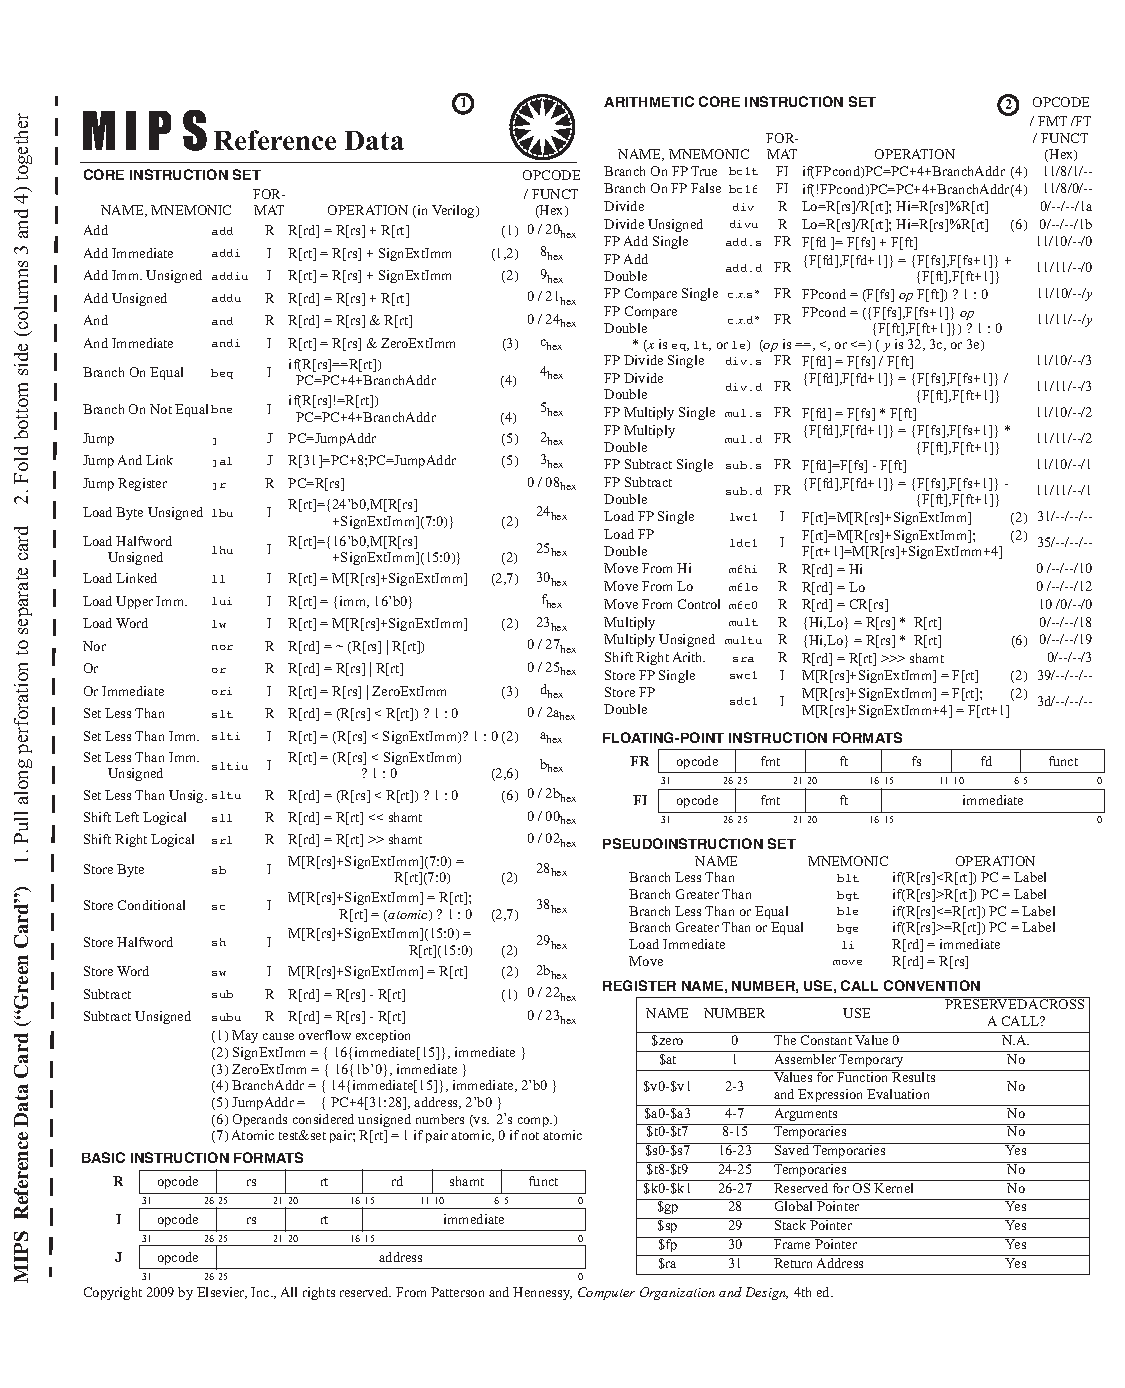
\includepdf[pages=-]{MIPS_Green_Sheet.pdf}
\showpoints
\end{document}
